\documentclass[a4paper, twocolumn]{ieee}
\usepackage[T1]{fontenc}
\usepackage[english]{babel}
\usepackage{amsmath}
\usepackage{graphicx}
\usepackage{verbatim}
\usepackage{titlesec}
\usepackage{float}
\setcounter{secnumdepth}{5}   
\setcounter{tocdepth}{5} 

% Hypertext
\usepackage{hyperref}

%Bibliobraphy
\usepackage{natbib}
\usepackage{bibtopic}
\usepackage{url}

\bibliographystyle{IEEEtran}
\bibliography{IEEEabrv,library}



\usepackage[utf8]{inputenc} % Krävs för att svenska tecken ska läsas korrekt i vissa system.
%\usepackage[latin1]{inputenc} % Om svenska tecken inte fungerar korrekt, försök att byta ut föregående rad mot denna (eller testa utan någon av raderna)

%Allow the use of \verbatimtabinput which includes external files, and handling tabs correctly
\usepackage{moreverb}
\def\verbatimtabsize{4\relax} 

\bibliographystyle{unsrt}

%Remove red boxes due to the hyperref
\hypersetup{
    colorlinks,
    citecolor=black,
    filecolor=black,
    linkcolor=black,
    urlcolor=black
}
%%%%%%%%%%%%%%%%%%%%%%%%%%%%%

\title{ETS200 -- Group K\\--\\ Final Report \\
How can web applications be tested?
%TODO maybe add a better title
}

\author{Fernando de Andrade Pereira
\\Jesper Bonna
\\Sadat Tokhi
%TODO put your full names, guys
}

\begin{document}
\maketitle
\thispagestyle{empty}
\clearpage

\begin{abstract}
With the growth in the industry of Web applications, specifc software testing techniques have been developed. 
However, it is facing a lot of challenges.

This paper describes techniques, tools, experiments, and the present and future in testing Web applications. 

\end{abstract}
\thispagestyle{empty}
\clearpage

\tableofcontents
\thispagestyle{empty}
\clearpage

\setcounter{page}{1}

\section{Introduction}
The World Wide Web has grown hugely in the last decades.
Over the years, static Web pages have become obsolete and several Web \emph{applications} have arose.

These Web application, as any other piece of software developed, shall be tested.
Many traditional software testing techniques  -- as \emph{white box} or \emph{black box} -- have been used.
However, these techniques are not completelly appropriate to test Web applicaton, due to dynamism of Web pages and communication between server and client sides.

In this paper, we'll analyse the adaptations that have been done in the traditional techniques to apply them in new Web applications, the several existing tools do this testing, a comparative study between different techniques and a brief consideration about the present and future of Web application software testing.

\section{White box testing on Web application}
The main idea with white box testing is to focus on the inner structure of the software \cite{ib03}. To do this
a tester needs to have access to the code or a pseudo like functionality representation of the code. A
coverage model is used to specify which parts of the code that needs to be tested. A commonly used
test model is a Control Flow Graph, shown below \cite{p91}:


\begin{figure}[H]
	\centering
	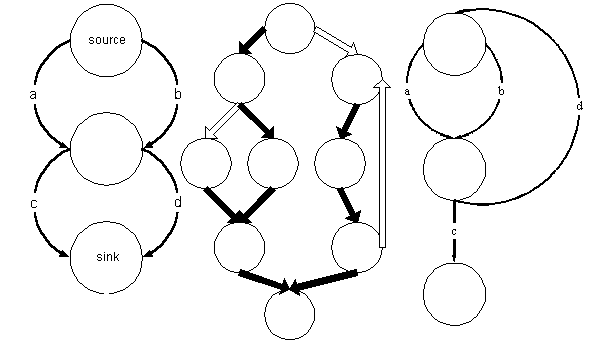
\includegraphics[scale=0.4]{fig.png}
	\caption{Simplified Control Flowgraph, Flowgraph with marked edges and Simplified Flowgraph with Looping}
\end{figure}



There are several different coverage models which serves different purposes \cite{ib03}. \emph{Statement coverage}
is model which executes and tests all statements in the code. Here logical faults in loops and if-
statements are often found. \emph{Condition coverage} tests all possible conditions, which covers the
variables possible values. \emph{Branch coverage} tests all possible paths throughout the system. Even
though the output might be the same for two executions it doesn’t necessarily have to take the same
path, and something else can cause an issue along the way.

To the code representation models that test Web applications, two main families of structural
models have been practiced from theory \cite{dlf06}. One model focuses on the level of abstraction of
single statements of code components of the application, and represents information about their
control flow or data flow. The other “family” focuses on the granularity of the pages from the Web
application and represents the navigation structure between pages of the application with some
eventual added details. Two techniques are proposed below:

Liu et al.\cite{lkhh01} has proposed a technique that shows example of how data flow testing of Web
applications can be carried out. The model can be used on applications implemented in HTML and
XML languages. This model is based on a Web application test model called WATM, which includes
and Object model and a Structure model. The purpose of the Object model is to represent the
ways that heterogeneous components are interconnected. There are three types of objects: client
pages, server pages and components. Relationships between objects are inheritance, aggregation,
association, request, response, navigation, and redirect. The first three have objected-oriented
semantics while the rest have has specific relationships between client and server pages. The
structural model uses four types of graph to cover various types of data flows of a Web application:
a \emph{Control Flow Graph} (CFG) of an individual function, the \emph{Interprocedural Control Flow Graph} (ICFG),
an \emph{Object Control Flow Graph} (OCFG), which integrates CFGs of object functions that are included in
sequences that are triggered by GUI events, and there is the \emph{Composite Control Flow Graph} (CCFG)
that covers the interaction between pages.

The approach of data-flow testing folders test cases into three different categories, intra-object,
inter-object and inter-client. These are then defined by five scopes of the testing level: Function,
Function Cluster, Object, Object Cluster, and Application level.

For the \emph{intra-object} perspective, test paths are selected for variables that have def-use chains within
an object. The chains are computed using the control flow graphs of functions included in the object.
The \emph{inter-object} test paths are selected for variables that have def-use chains across objects. Def-
use chains have to be defined at the \emph{object cluster} level, where each cluster is composed by a set of
message-passing objects. At last the \emph{inter-client} perspective derives test-paths on the basis of def-use
chains of variables that span over multiple clients, since in a Web application a variable can be shared
by multiple clients. This level of testing is called \emph{application} level.

The relevance in this test technique lies in its potential to extend the field of how Web applications in
the data flow testing approaches applicable to traditional software. Although its effectiveness is still
not great, further investigation in this area needs to be done for developers to consider using it. Also
there hasn’t been a validation including more than one example of Web application.

The other technique from the second “family” described earlier has been introduced by Ricca and
Tonella \cite{rt01}. The approach is based on HTML navigation links of the application. The same authors
presented a model called the Control Flow Model, which represents the internal structure of Web
pages where the execution flow is followed. This model has been used for structural testing as well.

In this model a test case is defined as a sequence of Web pages to be visited and the input values to
those pages with forms. This model includes branch coverage, path coverage and node coverage.

A conclusion regarding these different tests is that they serve different purposes. Some tests are
applicable at system integration level and other at a more detailed unit level. The first technique
proposed by Liu et al is applicable at a wide spectrum of testing levels. The intra-object covers unit
tests and the inter-object / inter-application covers the system integration. The Control Flow Model
by Ricca and Tonella can only be used at system level. As a tester who needs to test both at unit level
and system level the first model might have an advantage, since it is more practical sticking with one
model. Although the controversiallity regarding this model is a disadvantage.


\section{Tools for testing web applications}
%TODO Common tools for testing web based applications. When is each tool most useful?

 The number of tools that are available online for websites/applications has increased significantly in the last few years. There are too many tools to try and list and analyze them all so we have chosen a few that we will present briefly and try to explain when each of these tools is most useful. 
 Categorizing web tools is hard since many of the tools can be listed in several of the categories. These are some of the categories for web testing tools.  

 \begin {itemize}
 \item Load and performance test tools  
 \item Java test tools 
 \item Link checkers 
 \item Html validators 
 \item Web site security check tools 
 \item Mobile/Web app testing tools
 \end {itemize}
 
We have chosen one web testing tool in each category and they are presented in the same order as their categories. 
The tools were picked in a random manner and where in no way picked due to their performance in their respective area.
 
First up is a tool called \emph {Agileload} from Agile Load SA. Agileload is used for testing all web and mobile applications.
With Agileload the user can create different scenarios simulating heavy traffic in order to test the performance of the
application/website. Another feature of Agileload is its topological and thresholds analysis. These features are helpful 
in pinpointing the origin of anomalies. There are many more features to Agileload that the user can take benefit from.
Agileload is very versatile since
it supports
applications
running J2EE,
Ajax, Adobe Air-Flex, Silverlight, Sharepoint, JSON, 
Web services, SOAP, Apache, IIS, Web sphere, Jboss, Oracle, SQLServer, MySQL, DB2, SAP Web, Siebel, PeopleSoft, Hyperion, 
Citrix and
many more \cite{agileload}.
 
Next up is \emph{Autopilot Heap Detective} from Nastel technologies.
AHD is a free tool that's used for analyzing and detecting 
memory leaks in the java heap. It simply holds track of all objects on the heap and reports anomalies in the memory. \cite{ahd}
 
The next tool is \emph{LinkScan} from Electronic Software Publishing Co. The name reveals this tools main objective. It scans all 
links in an application/website and searches for broken/bad links and stores the results in a report in a database that the 
user can access in order to follow up and repair these links. \cite{links} 
 
\emph {Total Validator} is used for validating html and xhtml against the W3C CSS Standards \cite{w3}. Other features are searching 
for broken links and spellchecking. The spellchecker covers the following languages. American English, British English,
French, Italian, Spanish and German.\cite{totval} 

\emph {SkipFish} is a web security tool from Michael Zalewski/Google. It's main purpose is scanning websites/applications for 
security threats of all measures and helping the user to prevent against these threats. \cite{skipfish}
 
The last tool to be presented is\emph {MobiTest} from Mobile Performance Testing Tools.  With Mobitest the user can test the 
performance of their website by browsing it on mobile devices from different locations. The test data returns information 
on the site’s load time, bandwidth, charts, pictures and optionally video footage of the site. \cite{mobitest} 
 
 
As we mentioned before, categorizing web testing tools is hard. And from just these few examples that we just presented 
one can see that this is true. Many of the web testing tools are multifunctional and can be used for different kinds of 
tests. But still it seems as if just one tool won’t be sufficient for a user to fully test a website/application for all 
types of errors and bugs that can arise. Maybe this is because of the broad variety in styles, forms and different coding 
languages in modern day’s websites/applications.  Testing websites /applications is hard since there are so many inputs 
and outputs to handle, and many of today’s websites are dynamic pages, meaning that there are different inputs and outputs 
for different users making it harder for the developers of web testing tools to create a tool that can cover all error hecking.
  
Many of the web testing tools has the ability to set up and perform automated test cases, but this is mainly for tests 
concerning issues like checking for broken /bad links, simulating heavy traffic, testing a websites/applications load 
time, spellchecking etc. When it comes to test cases concerning interaction between a user and a website/application 
the user has to set up manual test cases.   
 
So in conclusion we would say that to fully test a website/application you would need more than a single tool. And even then 
there is no guarantee that it’s foolproof.  But for the average user the combination of using one or a few tools is 
sufficient to make their website/application somewhat error free and optimized.



\section{Case studie: AJAX web applications \cite{mtr08}}
%TODO Fernando: Which cases have been studied? Which technics have been applied? How can the results be evaluated?

AJAX is a technology that can be used to develop Rich Internet Applications.
Since it use assynchronous messages between client and server and it allows dynamic page alteration in a different way than the multipage Web paradigm, it introduces new chalenges to the testing of these web applications.

\subsection{Techniques}
In the paper \cite{mtr08}, four Web application testing techniques are introduced: \emph{model-based}, \emph{code-coverage-based}, \emph{black box} -- three tradicional Web applications testing techniques -- and \emph{state-based} -- this last one proposed as more adequate to handle with AJAX applications.

\subsubsection{Model-based testing}

It is a \emph{white box} testing technique.
A model of the application is constructed using reverse engineering and Web crawling technique -- a program that automatically transverses the Web's hyperlink structure, retrieving the content of the Web pages.
It generates a graph where the nodes represent pages and edges represent links.
The test cases will be defined chosing a coverage criteria and applying to this model. 

\subsubsection{Code-coverage-based testing} 

It is another \emph{white box} testing technique. 
It uses a control flow model of the application where nodes represent statements execute by the Web server or by the client and edges represent control transfer.
Theoretically, it can be use to test a AJAX Web application, but due to the complexity and dynamism of AJAX Web pages, this technique is very limited for this use.

\subsubsection{Black box testing} 

It uses functional requirements of the application to define test cases, i.e., scenarios that can be accomplished by a Web visitor through the browser.

\subsubsection{State-based testing}

It is proposed by the autors of the paper as a more efficient way of test a AJAX Web application.

Using AJAX, the state of the elements in the client-side can change dynamically.
A \emph{state} is considered a possible instance of the DOM in a Web page, i.e., it's characterized by the HTML elements.

A finite state machine describes the the behavior of the Web page, containing the states (equivalence classes can be used to reduce the total number of states) and the transitions, related to methods triggered by GUI events -- interations with the user, like button clicks -- and \emph{callback} functions -- tht happen when the page receive a response from ther server.

The method consists in: 

\begin{enumerate}
\item \emph{FSM construcion}. The FSM that models a AJAX Web page an be constructed during the design phase or can be reverse enginnered from the code.
\item \emph{Path extraction}. One coverage criteria (states or transitions coverage) is chosen and the paths are extracted from the FSM according to it.
\item \emph{Test cases generation}. Each path is converted into a test case.
\item \emph{Test cases execution}. A tool that works in HTTP request-response level is used execute the test. cases
\end{enumerate}

\subsection{Experiments}

The experiment consists in use the four testing techniques introduced to test two diffentent Web applications composed of Java, JSP and Javascript code -- \emph{Photoshare} and \emph{theOrganizer}.

\subsubsection{Preparation and procedure}

To test the \emph{effectiveness} of each technique, and the \emph{effort} demanded by them, faults are injected in the code of both applications (seven faults in \emph{Photoshare} and nine in \emph{theOrganizer}).
These faults try to simulate bugs commonly found in real applications and are introduced by a person different than the tester.

For each testing technique, a suite of test cases is defined.
This test cases suites are applied using following metrics:

\begin{itemize}

\item To test \emph{effectiveness}:
\begin{itemize}
\item number of faults revealed;
\item number of use cases exercised;
\item severity of faults -- the person who injected the faults determine each one as \emph{severe} or \emph{not severe} according to the potential tha it has to crash the system;
\item number of faults with high degree of relation with AJAX technology.
\end{itemize}

\item To test \emph{effort}:
\begin{itemize}
\item number of test cases in the suite;
\item complexity of the whole suite;
\item time needed (\emph{man-hours}) to prepate the testing environment.
\end{itemize}

\end{itemize} 

\subsubsection{Results and conclusion}

The \emph{state-based} and the \emph{blak box} techniques found thirteen faults each, and were the better techniques in this criterion.
However all the techniques seens to be complementary, since they find different errors in the systems.

As expected, the \emph{black box} technique is the one that covered more use cases, but not the whole set.
It covers 91\% of the total of use cases.

Eight of the total number of fault were considered \emph{severe}. Again, \emph{black box} testing and \emph{state-based} testing had the better results, finding 75\% of the \emph{severe} faults each.

There were eight \emph{AJAX related} faults among the total number of errors. 
\emph{State-based} testing found 75\% of these bugs, and was the better than the other techniques in this metric.

It's possible to conclude that the traditional techniques and \emph{state-based} testing are complementaries.
The \emph{state-based} testing is more likely to find errors related to AJAX, other techniques will work better with other kind of errors.

The \emph{state-based} testing is not the technique with the largest test cases suite (it has 78 test cases, against 111 of the \emph{code-coverage-based}, 93 of the \emph{black box} and 61 of the \emph{model-based}).
However it had the test suite with the biggest complexity in average and by far the technique that demands more time of preparation of the testing environment.

Summing up, although the \emph{state-based} testing technique demands a effort bigger than the traditional testing techniques, only it can reveal some faults related to the AJAX technology, due to be the only one that focuses it.
The traditional techniques, nevertheless can be used as complement to the proposed one, since they found errors that are difficult to find using \emph{state-based} testing.


\section{Analysis}

\subsection{Major problems with web-based testing today}
%TODO There is a lot of problems with web based testing today. Mostly it’s too time consuming and developers doesn’t have the time to test before release.
There are some factors that contributes to the difficulty of developing
generic web testing tools that can be used for testing any kind of
website/application and doing so without beeing to timeconsuming or
errorprone. The fact that different developers have different testing
strategies, there are different browsers, the wast range of programming
languages available, the dynamic nature of many websites/applications and
last but not least the unpredictable behavior of the users. 

All these
facts combined explains why web testing tools are not optimized, atleast
not yet. Because of this testing websites/applications is timeconsuming
since, in most cases, the user has to manualy setup test suits for
different kinds of testing scenarios. Sometimes it's impossible to test
all different testing scenarios due to the fact that there are so many
combinations of inputs/outputs. There is no solution to these problems yet
but in the next section, "what does the future hold", we discuss briefly
what is expected in the near future in order to make it a little easier
for developers aswell as for the users. \cite{dlf07}

\subsection{What does the future hold?}
%TODO How can strategies and method

In the future there is a demand for tools that has greater support for testing dynamic websites/applications, tools 
with greater support for automated test cases, tools that can reuse statistical test suites that covers common ground 
and tools that are able to properly test new technologies. Lately more and more web testing tools are being developed
as web services. This means that the testing strategies and methods that exist for web testing tools today has to be 
adapted to the new approach of web services.\cite{dlf07} For the interested reader there is a website listing and linking to over
200 web testing tools amongst others the ones that we have presented. \cite{softqa}


\appendix

\section{References}

\begin{btSect}[plain]{literature}
\subsection{Articles \& books}
\btPrintAll
\end{btSect}

\begin{btSect}[plain]{websites}
\subsection{Websites}
\btPrintAll
\end{btSect}

\end{document}
